% TeX root=../main.tex

\section{Concordância}

Adjetivos concordam em gênero, número e caso com seu
substantivo.
Adjetivos modificando um possessor expresso por um adjetivo de posse em
\emph{-asi-} concordam com o adjetivo de posse:

\exg. \emph{wasu-s} \emph{Runtiy-asi-s} \emph{nimuwiza-s}\\
bom-\Nom\Sg\Com{} R.-\emph{poss.}-\Nom\Sg\Com{} filho-\Nom{}\Sg\Com{}\\
o filho do bom Runtiya \emph{ou} bom filho de Runtiya


\noindent Verbos concordam com o sujeito em número e pessoa.

Verbos com seu sujeito no neutro plural podem permanecer no singular:

\exg. \emph{katin-a} \emph{wasuw-a} \emph{as-ti}\\
vasilha-\Nom\Pl\Neut{} bom-\Nom\Pl\Neut{} ser-3\Sg\textsc{Ind.Pres.}\\
as vasilhas são boas


\noindent Numerais acima de um podem modificar substantivos no singular.


\section{Uso dos casos}

\paragraph{Nominativo}
Caso do sujeito e predicativo do sujeito.
Orações predicativas na maioria das vezes não utilizam o verbo \emph{as-} `ser'.

\exg.\emph{katin-a} \emph{wasuw-a} (\emph{as-ti})\\
vasilha-\Nom\Pl\Neut{} bom-\Nom\Pl\Neut{} (ser-3\Sg\textsc{Ind.Pres.})\\
as vasilhas são boas


\paragraph{Acusativo}
Expressa normalmente o objeto direto da oração.
Outros usos incluem:
\begin{inparaenum}[(a)]
	\item duplo acusativo:
	\emph{amu=pa=wa=\textbf{n} zadi \textbf{istran} daha}
	`aqui eu \textbf{o} peguei \textbf{pela mão}'\footnote{KARKAMIŠ A7, §3.};
	\item duração de tempo: \emph{\logo{`ANNUS'}-an \logo{ANNUS}-an} `ano após
	ano'.
\end{inparaenum}
\clearpage


\paragraph{Genitivo}
Expressa posse e pode ser substituído pelo adjetivo de posse em \emph{-asi-} e a
pluralidade apenas pode ser entendida a partir do adjetivo de posse:\footnote{
Há dois exemplos de inscrições provenientes de Commagene da idade do ferro em
que um genitivo em \emph{-as{(i)}} parece expressar pluralidade do possessor,
a saber, ANCOZ 7, §4 (\citeabbrev*{CHLI12}, p.\ 356) e GELB, §1
(\citeabbrev*{CHLI12}, p.\ 569). Há sinais em luvita cuneiforme de que formas
propriamente pluralizadas de adjetivos possessivos tenham sido
produzidas~\citep[pp. 45ff.]{Yakubovich2010}.
}

\ex.\ag.\emph{tati-s} \emph{masan-inzi}\\
pai-\Gen\Sg\Com{} deus-\Nom\Pl\Com{}\\
os deuses do pai
\bg.\emph{tat-as-inzi} \emph{masan-inzi}\\
pai-\emph{poss.}-\Nom\Pl\Com{} deus-\Nom\Pl\Com{}\\
os deuses dos pais\slash{}do pai\slash{}paternos


\paragraph{Dativo--Locativo}
Expressa tanto o objeto indireto do verbo quanto o local em que a ação verbal
ocorre. Outros valores semânticos podem ser expressos pelo dativo:
\begin{inparaenum}[(a)]
	\item dativo de posse\slash{}interesse:
	\emph{a=wa=\textbf{ti} alamanza izisatai}
	`ele
	honra o nome \textbf{para si} $\rightarrow$ ele honra \textbf{seu próprio}
	nome';\footnote{KARKAMIŠ A1\emph{b}, §2.}
	\item  direção\slash{}alativo:
	\emph{\textbf{apatanza}=pa=wa=ta \textbf{walilidanza} aminzi tatinzi
	huhanzi=ha {?}-linzi=ha na hwi\-hwisantasi}
	`Meus pais, avôs e bisavôs não marcharam \textbf{para estes
		territórios}';\footnote{KARKAMIŠ A11\emph{b}+\emph{c}, §8.}
	\item dativo de comparação: Ver~\autoref{sec:Comparacao};
	\item tempo em que algo ocorre: \emph{apa\-di \logo{ANNUS}-usi} `naquele ano';
	\item objeto de infinitivos (raro).
\end{inparaenum}


\paragraph{Ablativo--Instrumental}
Expressa lugar de origem de um movimento, separação ou instrumento de uma ação.
Outros usos incluem:
\begin{inparaenum}[(a)]
	\item causa de um evento:
	\emph{a=wa=mu amis nanis Tarhuntas, Karhuhas, Kubabas=ha
		\textbf{amiyati tara\-wanidi} azanta}
	`E \textbf{por causa da minha justiça}, meus senhores Tarhunta, Kar\-huha e
	Kubaba me amaram';\footnote{KARKAMIŠ A11\emph{a}, §7.}
	\item agente da passiva: \emph{\textbf{masanadi} azamis hantawatis}
	`rei amado
	\textbf{pelos deuses}'.
\end{inparaenum}

\section{Posposições}
Diferentemente do português, o luvita possui posposições.
Salvo a posposição \emph{arha} `para longe de', que recebe ablativo, todas as
preposições recebem dativo.

\clearpage
\section{Comparação}\label{sec:Comparacao}
A comparação pode ser construída por dois dispositivos sintáticos:
\begin{compactenum}[(a)]
	\item adjetivos seguindo \emph{\logo{FRONS}-li- = hantili-} `o mais X':\\
	\emph{hantili \logo{ARGENTUM.DARE}-siya}\\ `o mais caro'\footnote{KARKAMIŠ
		A11\emph{a}, §17.}
	\item Subst$_{1,i}$ -- Subst$_{2,\emph{dat.}}$ --- Adj$_i$ = `Subst$_1$ é mais Adj que Subst$_2$':\\
	\emph{apas=wa=\uwave{mu} \uline{lananza} \textbf{uran}  izida}\\
	`ele \uwave{me} fez \textbf{maior} que os \uline{irmãos}'\footnote{TEL
		AHMAR 1, §16.}
\end{compactenum}


\section{Advérbios}
Além dos advérbios produzidos a partir dos pronomes relativos e demonstrativos,
pode-se produzir advérbios a partir de adjetivos utilizando o acusativo neutro
de qualquer adjetivo: \emph{wasu usanusaha} `eu me aproveitei
bem'.\footnote{BULGARMADEN, §8.}


\section{Ordem de palavras}\label{sec:Ordem}

Via de regra, a ordem de palavras `não-marcada' é sujeito--objeto--verbo (SOV).
Os pronomes relativos e outros complementizadores ocorrem no meio da sentença.
Pronomes relativos, em geral, seguem o sujeito.\footnote{Ainda é necessário um
	estudo mais específico sobre ordem de palavras e orações relativas,
	pessoalmente acho pouco convincente essa regra.}
Pronomes interrogativos ocorrem em primeira posição, normalmente.
A negação precede o elemento negado ou, caso o escopo seja a oração por completo,
o a sequência de prevérbio + verbo.

\section{Orações interrogativas}
Como mencionado em~\autoref{sec:Ordem}, orações interrogativas abertas -- i.e.\
que contém um pronome interrogativo -- são iniciadas pelo pronome da série
\emph{kwi-}.
Orações interrogativas polares -- i.e.\ de sim e não -- devem ser identificadas
pelo contexto.

\section{Coordenação}
As partículas adversativa \emph{=pa} e aditiva \emph{=ha} são mutualmente
exclusivas.
O assíndeto é comum tanto quando a coordenação ocorre no escopo oracional quanto
no escopo de dois ou mais substantivos.
Para conectar dois ou mais substantivos, a partícula \emph{=ha} é adicionada ao
último elemento ou a todos os elementos menos o primeiro.

\ex.\ag.\emph{Tarhuntas} \emph{Karhuhas} \emph{Kubabas=ha}\\
T. K. K.=\Conj{}\\
Tarhunta, Karhuha e Kubaba\footnote{KARKAMIŠ A11\emph{a}, §7.}
\bg.\emph{tatinzi} \emph{huhanzi=ha} \emph{{?}-linzi=ha}\\
pais avôs=\Conj{} bisavôs=\Conj{}\\
pais, avôs e bisavôs\footnote{KARKAMIŠ A11\emph{b}+\emph{c}, §8.}


\noindent Caso o último elemento seja composto por múltiplas palavras, \emph{e.g.}
adjetivo + substantivo, a coordenação se apoia no primeiro elemento:


\exg.\emph{tipasis} \emph{Tarhunzas,} \emph{tipasis} \emph{Tiwazas,} \emph{Iyas,} \emph{taniminzi=ha} \emph{masaninzi}\\
celeste T. celeste T. I. todos=\Conj{} deuses\\
o celete Tarhunza, o celete Tiwada, Ea e todos os deuses\footnote{KARATEPE 1,
	§LXXIII, Hu.}


\section{Subordinação}
Como mencionado em~\autoref{sec:Ordem}, partículas de
complementizadores\slash{}subor\-di\-na\-do\-res ocorrem no meio da sentença, por vezes
como última palavra.
A parataxe, no entanto, é comum.

\paragraph{Causais}
As conjunções causais são \emph{kwari}, \emph{kwanza} e \emph{kuman}, os verbos
ocorrem no indicativo.

\ex.\a. \emph{na=wa=n \textbf{kwari} pitahaliyaha\ldots{}}\\
Porque eu não o adquiri\ldots{}\footnote{KARKAMIŠ A11\emph{b}+\emph{c}, §31.}
\b.\emph{taruwis=pa=wa=mu=ta \textbf{kwanza} zatiyanza haristananza apan awida\ldots{}}\\
Porque a madeira para estes andares superiores veio
depois\ldots{}\footnote{KARKAMIŠ A11\emph{b}+\emph{c}, §33.}
\b. \emph{a=wa=ri \textbf{kuman} hatura\ldots{}}\\
Já que você (deve) escrever\ldots{}\footnote{ASSUR \emph{f+g}, §11.}



\paragraph{Condicionais}
As conjunções condicionais são \emph{kwadi\slash{}kwari}.
O verbo da apódose (resultado da condição) pode aparecer tanto no presente do
indicativo quanto no imperativo enquanto o verbo da prótese (condição) sempre é
atestado no indicativo presente.

\ex.\emph{hantawatadi=pa=wa \textbf{kwari} kwis=ha \ldots{} za asazaya \ldots{},
	a=wa=ta arha itintu\linebreak tipasis Tarhunzas, tipasis Tiwazas, Iyas,
	taniminzi=ha masaninzi hantawata\-hisa apan=ha hantawatin, apan=ha=wa
	\logo{CAPUT}-in.}\\
Se alguém entre os reis (\ldots{}) proclamar o seguinte (\ldots{}), que o celeste
Tarhun\-za,
o celeste Tiwaza, Ea e todos os deuses apaguem totalmente o reino e este rei e
este homem.\footnote{KARATEPE 1, §§LIX--LXXIII, Hu.}


\paragraph{Concessivas}
As conjunções concessivas são \emph{kwi} e \emph{kwa\emph{(}n\emph{)}za}.

\ex.\a.\emph{Kamanis=pa=wa \textbf{kwi} nirawanis asta\ldots{}}\\
Embora Kamanis fosse criança\ldots{}\footnote{KARKAMIŠ A6, §18.}
\b.\emph{nirawanis=wa=sa \textbf{kwanza} asta\ldots{}}\\
Embora ele fosse criança\ldots{}\footnote{KARKAMIŠ A7, §5.}


\paragraph{Consecutivas}
A conjunção consecutiva é \emph{kwati} `de modo que, para que'.

\ex.\emph{kwipa=wa=ta arlantanza apatanza harnisa anta tamaha,
	Adanawas=\linebreak=wa
	\textbf{kwa\-ti} warayamala asai}\\
Então eu construí fortalezas naqueles lugares, de modo que Adanawa\linebreak
ficasse em paz.\footnote{KARATEPE 1, §§XXIII--XXIV, Hu.}

\paragraph{Relativas}
As orações utilizam toda a série do pronome relativo \emph{kwi-}.
Em geral o pronome está posicionado logo depois do sujeito (ver nota acima).

\ex.\emph{haniyataya=pa=wa \textbf{kwaya} taskwiri anda asta, a=wa=ta
	taskwiriri arha par\-haha}\\
Mas os males que haviam dentro do território, eu os expulsei do
território.\footnote{KARATEPE 1, §§XII--XIII, Hu.}

\paragraph{Temporais}
A conjunção temporal é \emph{kwi} `quando'

\ex.\emph{aminzi=ha=wa tatinzi huhanzi=ha \textbf{kwi} azusataluna {\ldots}
	\logo{PES\textsubscript{2}.PES\textsubscript{2}}-danta,\linebreak kwipa=wa Runtiyas na
	kwishan wariyata.}\\
E quando meus pais e avôs iam cavalgar, de fato Runtiya não
os ajudou de modo algum.\footnote{BOHÇA, §10--11.}

\clearpage



\section{Leitura: BOHÇA}


A inscrição (\autoref{fig:bohça}) é conhecida desde 1901, tendo sido encontrada
em uma colina do vilarejo de Bohça (Bozca ou Bahçeköy),
provavelmente no contexto original e está atualmente locada no Kayseri
Arkeoloji Müzesi (no.\ 6).
O governante Kurtis filho de Ashwisis talvez possa ser identificado com o
mesmo governante mencionado por Sargão II por Kurti de Atunna entre 718--713
\textsc{aec}, e o estilo da inscrição corresponde ao esperado para este
período.
A associação, no entanto, depende da localização de Atunna.
Bohça está no meio da região conhecida das fontes
neo-assírias pelo nome de Tabal que, na idade do ferro, era composta por
diversas pequenas cidades-estado.

\begin{center}
	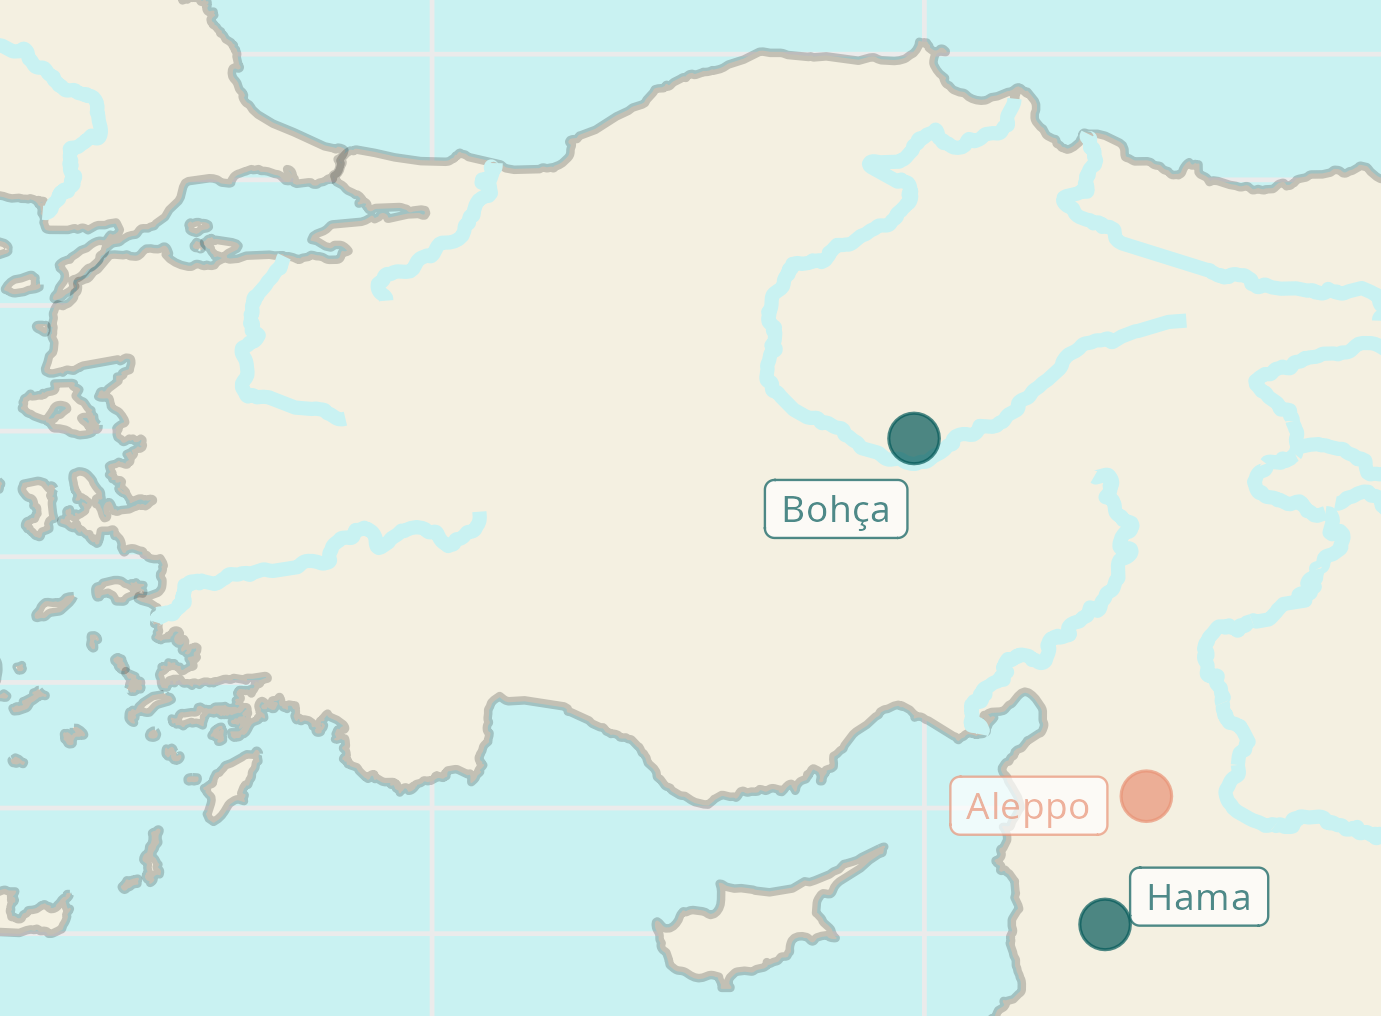
\includegraphics[width=0.65\textwidth]{../../../Mídia/Map03.png}
\end{center}


\begin{figure}[h]
	\centering
	\begin{subfigure}{0.49\textwidth}
		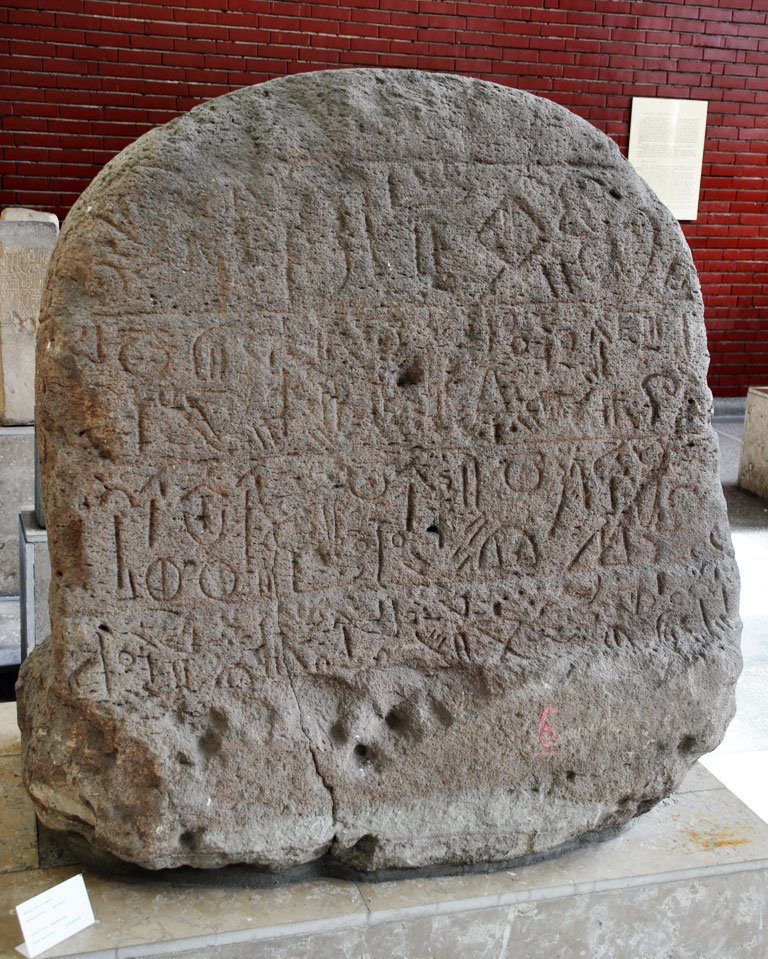
\includegraphics[width=0.9\textwidth]{../../../Mídia/bahce08.jpg}
	\end{subfigure}
	\hfill
	\begin{subfigure}{0.49\textwidth}
		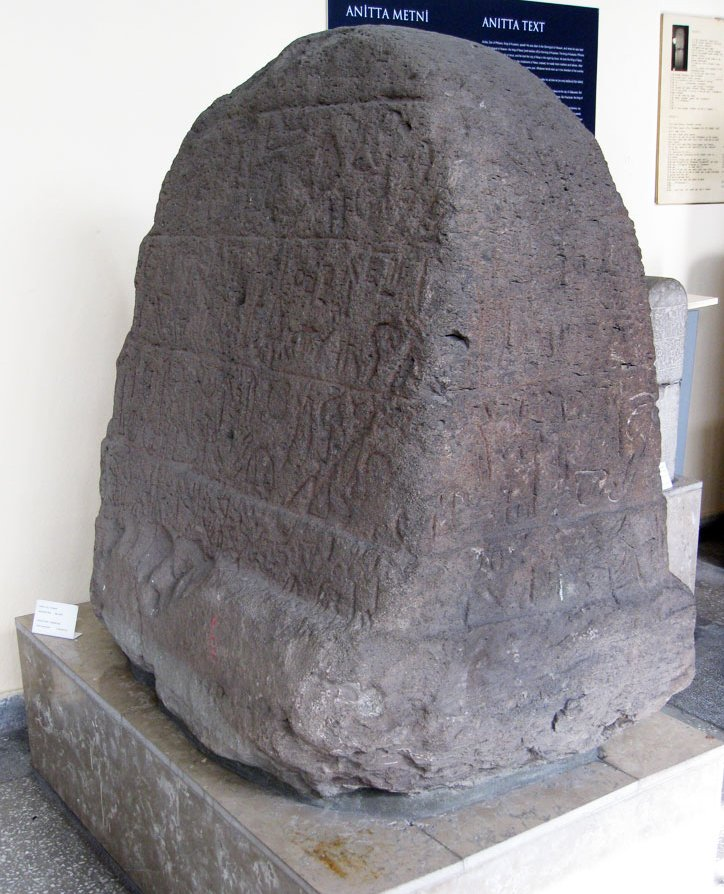
\includegraphics[width=0.9\textwidth]{../../../Mídia/bahce10.jpg}
	\end{subfigure}
	\caption[BOHÇA]{Inscrição BOHÇA. Dimensões da inscrição:
		1.26\times0.63m.
		Imagens de Cüneyt Süer, 2011,
		disponíveis em
		\href{https://www.hittitemonuments.com/bahcekoy/}{Hittite Monuments}.
		Edição e traçado em~\citeabbrev*{CHLI11}, pp.\ 478ff.\ e \emph{plate}
		265.
	}\label{fig:bohça}
\end{figure}

\clearpage

\begin{center}
	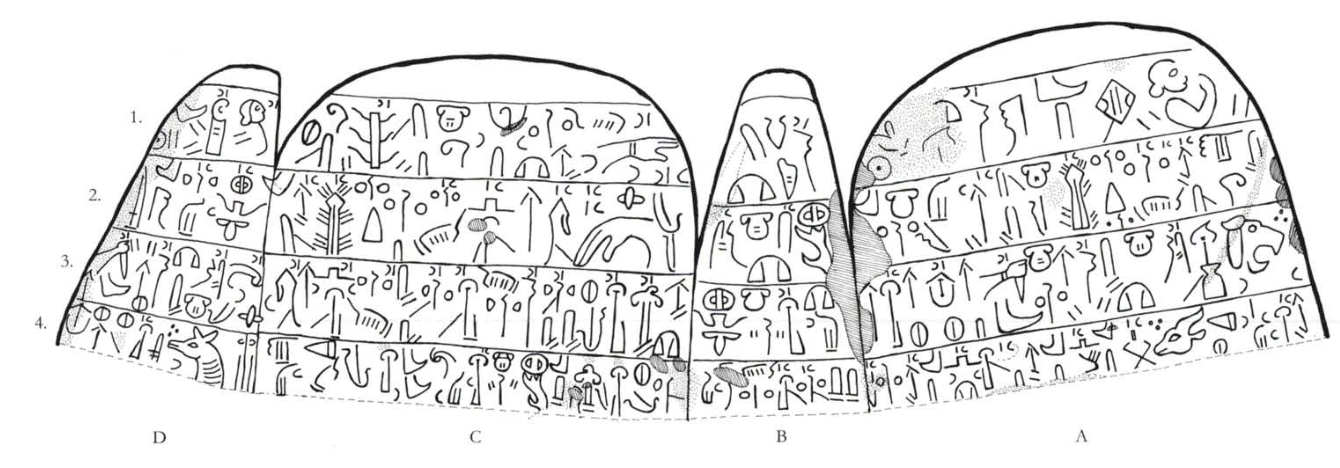
\includegraphics[width=\textheight,angle=90]{../../../Mídia/bohça.png}
\end{center}



\clearpage
\begin{parnumbersa}[]
	\raggedright%

	\Large \luwiantrans{EGO-mi}\hspace{5pt}
	[\luwmasc]\luwiantrans{ku-ra-ti-i-sá}\hspace{5pt}
	\luwmasc\luwiantrans{á-[sa-hwi-si]-sa4}\hspace{5pt}
	\luwmasc\luwiantrans{HEROS-li-i-sa}\hspace{5pt}
	\luwmasc\luwiantrans{<FILIUS>-ni-mu-wi-za-sa}\hspace{5pt}
	\luwiantrans{<OCCIDENS>-i-pa-ma-i+ri-i}\hspace{5pt}
	\luwmasc\luwiantrans{ORIENS-mi-ma-i+ri-ha}\hspace{5pt}
	\luwmasc\luwiantrans{PRAE}\hspace{5pt}
	\luwmasc\luwiantrans{AUDIREMI-ti-mi-sa4}\hspace{5pt}
	[\luwmasc]\luwiantrans{REX-ti-sá}\hspace{5pt}

	\Large \luwmasc\luwiantrans{wa-ta}\hspace{5pt}
	\luwmasc\luwiantrans{DEUS-TONITRUS-hu-ti}\hspace{5pt}
	\luwmasc\luwiantrans{za-i+ri}\hspace{5pt}
	\luwmasc\luwiantrans{BONUS-wa-su-wa-i}


	\Large \luwmasc\luwiantrans{wa-mu}\hspace{5pt}
	\luwmasc\luwiantrans{TERRA-REL-ra-zi}\hspace{5pt}
	\luwmasc\luwiantrans{SUPER-ra}\hspace{5pt}
	\luwmasc\luwiantrans{<CAPERE>-lu-na-'}\hspace{5pt}
	\luwmasc\luwiantrans{pi-pa-sa-i}\hspace{5pt}


	\Large \luwmasc\luwiantrans{DEUS-CERVUS3-ti-pa-wa-ta-'}\hspace{5pt}
	\luwmasc\luwiantrans{za-i+ri-ia-pa-a}\hspace{5pt}
	\luwmasc\luwiantrans{BONUS-wa-su-wa-i}


	\Large\luwmasc\luwiantrans{wa-mu}\hspace{5pt}
	\luwmasc\luwiantrans{za-ri+i}\hspace{5pt}
	\luwmasc\luwiantrans{sà-ma-ia}\hspace{5pt}
	\luwmasc\luwiantrans{<ANIMA-LEO>-hwi-sa5-ra}\hspace{5pt}
	\luwmasc\luwiantrans{pi-pa-sa-ia}


	\Large\luwmasc\luwiantrans{á-mi-zi-pa-wa}\hspace{5pt}
	\luwmasc\luwiantrans{tá-ti-zi-i}\hspace{5pt}
	\luwmasc\luwiantrans{AVUS-ha-zi-ha}\hspace{5pt}
	\luwmasc\luwiantrans{REL-zi}\hspace{5pt}
	[\luwmasc]\luwiantrans{sa-ta}\hspace{5pt}


	\Large\luwmasc\luwiantrans{REL-pa-wa}\hspace{5pt}
	\luwiantrans{DEUS-TONITRUS-hu-za-sa}\hspace{5pt}
	\luwmasc\luwiantrans{NEG2}\hspace{5pt}
	\luwmasc\luwiantrans{REL-ha-na}\hspace{5pt}
	\luwmasc\luwiantrans{wa-ra-ia-ia}\hspace{5pt}


	\Large\luwmasc\luwiantrans{á-mu=wa}\hspace{5pt}
	\luwmasc\luwiantrans{REL-ra}\hspace{5pt}
	\luwmasc\luwiantrans{wa-ra-ia-ia}\hspace{5pt}



\end{parnumbersa}

\vspace{10pt}
\hrule
\vspace{10pt}

\setcounter{parcount}{0}
\begin{parnumbersa}[]

	\raggedright%
	\itshape%

	\logo{EGO}-mi
	$[$\lmasc\textsuperscript{?}$]$ku+ra/i-ti-i-sá
	\lmasc{}á-[sa-hwi/a-si]-sa\textsubscript{4}
	\lmasc{}\logo{HEROS}-li-i-sa
	\lmasc{}\logo{``FILIUS''}-ni-mu-wa/i-za-sa
	\logo{``OCCIDENS''}i-pa-ma-ri+i-i
	\lmasc{}\logo{ORIENS}+MI-ma-ri+i-ha
	\lmasc{}\logo{PRAE}
	\lmasc{}\logo{AUDIRE}+MI-ti-mi-[sa\textsubscript{4}]
	\lbreak{} $[$\lmasc$]$\logo{REX}-ti-sá


	\lmasc{}wa/i-ta
	\lmasc{}\logo{DEUS.TONITRUS}-hu-ti
	\lmasc{}za-ri+i
	\lmasc{}BONUS-wa/i-su-wa/i-i


	\lmasc{}wa/i-mu
	\lmasc{}\logo{TERRA}-kwi+ra/i-zi
	\lmasc{}\logo{SUPER}+ra/i
	\lmasc{}\logo{``CAPERE''{(-)}}lu/a/i-na-'
	\lmasc{}pi-pa-sa-i


	\lmasc\logo{DEUS.CERVUS\textsubscript{3}}-ti-pa-wa/i-ta-'
	\lmasc{}za-ri+i{(-)}ia{(-)}pa-a
	\lmasc\logo{BONUS}-wa/i-su-wa/i-i


	\lmasc{}wa/i-mu
	\lmasc{}za-ri+i
	\lmasc{}sà-ma-ia
	\lbreak{}\lmasc{}\logo{``ANIMA.LEO''}-hwi/a-sa\textsubscript{5}+ra/i
	\lmasc{}pi-pa-sa-ia


	\lmasc{}á-mi-zi-pa-wa/i
	\lmasc{}tá-ti-zi-i
	\lmasc\logo{AVUS}-ha-zi-ha
	\lmasc{}\logo{REL}-zi
	$[$\lmasc\textsuperscript{?}$]$sa-ta


	\lmasc{}\logo{REL}-pa-wa/i \logo{DEUS.TONITRUS}-hu-za-sa
	\lmasc{}\logo{NEG\textsubscript{2}}
	\lmasc{}\logo{REL}-ha-na
	\lmasc{}wa/i+ra/i-ia-ia


	\lmasc{}á-mu-wa/i
	\lmasc{}\logo{REL}+ra/i
	\lmasc{}wa/i+ra/i-ia-ia



\end{parnumbersa}

\vspace{10pt}
\hrule
\vspace{10pt}


\setcounter{parcount}{0}
\begin{parnumbersa}[]

	\raggedright%
	\itshape%

	amu=mi Kurtis, Ashwisis \logo{HEROS}-lis nimuwizas,
	ipamari kistamari=ha paran tumantimis hantawatis.

	*a=wa=ta Tarhunti zari wasuwi,

	*a=wa=mu taskwirinzi sara luna pipasai.

	Runt{(iy)}i=pa=wa=ta zari {??} wasuwi,

	*a=wa=mu zari samaya hwisara pipasaya.

	aminzi=pa=wa tatinzi huhanzi=ha kwinzi *asata,

	kwipa=wa Tarhunzas na kwishan wariyaya,

	amu=wa kwari wariyaya:


\end{parnumbersa}

\vspace{10pt}
\hrule
\clearpage



\begin{parnumbersa}[]
	\raggedright%

	\Large\luwmasc\luwiantrans{wa-mu}\hspace{5pt}
	\luwmasc\luwiantrans{TERRA-REL-ra-zi}\hspace{5pt}
	\luwmasc\luwiantrans{SUPER-ra}\hspace{5pt}
	\luwmasc\luwiantrans{<CAPERE>-lu-na-'}\hspace{5pt}
	\luwmasc\luwiantrans{pi-pa-sa-i}\hspace{5pt}


	\Large \luwiantrans{á-mi-zi-ha-[wa]}\hspace{5pt}
	\luwmasc\luwiantrans{tá-ti-zi}\hspace{5pt}
	\luwiantrans{AVUS-ha-zi-ha[-']}\hspace{5pt}
	\luwmasc\luwiantrans{REL-i}\hspace{5pt}
	\luwiantrans{<ANIMA.EQUUS[>]-zú-sà-ta-la-u-na}\hspace{5pt}
	\luwmasc\luwiantrans{REL}\hspace{5pt}
	\luwmasc\luwiantrans{<PES2PES2>-da-ta}


	\Large\luwmasc\luwiantrans{REL-pa-wa}\hspace{5pt}
	\luwiantrans{DEUS-CERVUS3-ti-ia-[sá]}\hspace{5pt}
	[\luwmasc]\luwiantrans{NEG2-a}\hspace{5pt}
	[\luwmasc]\luwiantrans{REL-ha-na}\hspace{5pt}
	\luwmasc\luwiantrans{wa-ra-[ia]-ta}\hspace{5pt}


	\Large[\luwmasc]\luwiantrans{á-mu-wa}\hspace{5pt}
	\luwmasc\luwiantrans{REL-ra}\hspace{5pt}
	\luwmasc\luwiantrans{wa-ra-ia-ia}\hspace{5pt}


	\Large[\luwmasc]\luwiantrans{[a]-wa}\hspace{5pt}
	\luwmasc\luwiantrans{za-ti-i}\hspace{5pt}
	\luwmasc\luwiantrans{TERRA-sa-REL-ra-i}\hspace{5pt}
	\luwmasc\luwiantrans{za-ti-i}\hspace{5pt}
	\luwmasc\luwiantrans{LOCUS-lá-ti-i}\hspace{5pt}
	\luwiantrans{1 CENTUM}\hspace{5pt}
	\luwiantrans{ANIMA-CAPRA}\hspace{5pt}
	\luwmasc\luwiantrans{la-ha}\hspace{5pt}
	\luwmasc\luwiantrans{<UNUS>-ta}\hspace{5pt}
	\luwmasc\luwiantrans{REL-za}\hspace{5pt}



\end{parnumbersa}

\vspace{10pt}
\hrule
\vspace{10pt}

\setcounter{parcount}{8}
\begin{parnumbersa}[]

	\raggedright%
	\itshape%

	\lmasc{}wa/i-mu
	\lmasc{}\logo{“TERRA”}-kwi+ra/i-zi \logo{SUPER}+ra/i
	\lmasc{}\logo{“CAPERE”}{(-)}lu\logo/a/i-na
	\lmasc{}pi-pa-sa-ia


	\lmasc{}á-mi-zi-ha<-wa/i>
	\lmasc{}tá-ti-zi
	\lbreak{} \logo{AVUS}-ha-zi-ha-a?
	\lmasc{}\logo{REL}-i
	\logo{“ANIMA.EQUUS<”>}-zú-sà-ta-la-u-na
	\logo{REL}
	\logo{“PES\textsubscript{2}.PES\textsubscript{2}”}{(-)}da-ta


	\lmasc{}\logo{REL}-pa-wa/i
	\logo{DEUS.CERVUS\textsubscript{3}}-ti-ia-\textsc{⌈}sá\textsuperscript{?}\textsc{⌉} $[$\lmasc{}\textsuperscript{?}$]$\logo{NEG\textsubscript{2}}-a
	$[$\lmasc{}\textsuperscript{?}$]$\logo{REL}-ha-na
	$[$\lmasc{}\textsuperscript{?}$]$wa/i+ra/i-[ia?]-ta

	$[$\lmasc{}\textsuperscript{?}$]$á-mu-wa/i
	\lmasc{}\logo{REL}+ra/i
	\lmasc{}wa/i+ra/i-ia-ia


	\lmasc{}\textsc{⌈}a\textsuperscript{?}\textsc{⌉}-wa/i
	\lmasc{}za-ti-i
	\lmasc{}\logo{“TERRA”}-sa-kwi+ra/i-i
	\lmasc{}za-ti-i
	\lmasc{}\logo{LOCUS}-lá/í-ti-i \logo{1\times{}CENTUM} \logo{ANIMA.CAPRA} la-ha
	\logo{“UNUS”}-ta
	\lmasc{}\logo{REL}-za


\end{parnumbersa}

\vspace{10pt}
\hrule
\vspace{10pt}


\setcounter{parcount}{8}
\begin{parnumbersa}[]

	\raggedright%
	\itshape%

	*a=wa=mu taskwirinzi sara luna pipasai

	aminzi=ha=wa tatinzi huhanzi=ha kwi azusataluna {??}
	\logo{PES\textsubscript{2}.PES\textsubscript{2}}-danta,

	kwipa=wa Runtiyas na kwishan wariyata.

	amu=wa kwari wariyaya

	a=wa zadi taskwiri zadi arlanti $100$ sasanzi laha \logo{UNUS}-ta kwanza \ldots{}

\end{parnumbersa}

\vspace{10pt}
\hrule


\subsubsection*{Notas}

\paragraph{5}
\textbf{samaya} `?': há três interpretações para o termo:
\begin{inparaenum}
	\item a palavra é um substantivo neutro plural, agindo como aposto de
	\emph{hwisara} `animais selvagens, feras' e está associada a
	\emph{samanza} `selos' (KULULU 2, §2), talvez um substantivo derivado do
	verbo \emph{sa-} `selar, imprimir',
	dando o sentido de `ele me concede as feras, o combinado'.
	\item a palavra é um substantivo dativo singular, possivelmente derivado do
	mesmo verbo \emph{sa-} `selar, imprimir' com o sentido associado de
	`marcar $\rightarrow$ atirar, ferir', dando o sentido de `ele me deu as
	feras para ferir\slash{}atirar'.
	\item a palavra é um adjetivo concordando com \emph{hwisara}, sem sentido
	conhecido, talvez um plural neutro de \emph{sami-} `atirado, ferido'.
\end{inparaenum}

\bigskip
\noindent \textbf{Tradução}\\
\noindent [1] Eu sou Kurtis, filho do herói Ashwisis, rei conhecido do
pelo ocidente e oriente.

\noindent [2] Aqui eu sou bom para Tarhunta [3] e ele me
permite tomar (os) territórios.
[4] E aqui eu sou bom para Runtiya [5] e ele me concede (as) feras SAMAYA\@.

\noindent [6] Mas àqueles que foram meus pais e avôs [7] de fato Tarhunta não
ajuda de modo algum, [8] como ele me ajuda: [9] ele me permite tomar (os)
territórios.

\noindent [10] E quando meus pais e avôs iam cavalgar, [11] de fato Runtiya não
os ajudou de modo algum, [12] como ele me ajuda: [13] aqui em (seu) território,
aqui em (seu) lugar, capturei cem gazelas de uma vez \ldots

\bigskip
\begin{multicols}{2}[\noindent\textbf{Vocabulário}]
	\begin{hangparas}{1em}{1}
		\raggedright%
		\textbf{\emph{arlant-}} (\emph{subst.neut.}) \tabto{1em} lugar\\
		\textbf{\emph{Ashwisi}-} (NP) \tabto{1em} Ashwisis\\
		\textbf{\emph{azusatala}-} (\emph{v.i.}) \tabto{1em} andar a cavalo, cavalgar\\
		\textbf{\emph{\emph{HERO}-li}-} (NP) \tabto{1em} herói\\
		\textbf{\emph{huha}-} (\emph{subst.com.}) \tabto{1em} avô\\
		\textbf{\emph{hwisar}-} (\emph{subst.neut.}) \tabto{1em} fera, animal selvagem\\
		\textbf{\emph{ipami}-} (\emph{subst.com.}) \tabto{1em} ocidente\\
		\textbf{\emph{kistami}-} (\emph{subst.com.}) \tabto{1em} oriente\\
		\textbf{\emph{Kurti}-} (NP) \tabto{1em} Kurtis\\
		\textbf{\emph{kwi}} (\emph{adv.}) \tabto{1em} quando\\
		\textbf{\emph{kwipa}} (\emph{adv.}) \tabto{1em} de fato\\
		\textbf{\emph{la}-} (\emph{v.t.}) \tabto{1em} tomar\\
		\textbf{\emph{na kwishan}} (\emph{adv.}) \tabto{1em} de modo algum\\
		\textbf{\emph{paran tumanti}-} (\emph{v.t.}) \tabto{1em} ouvir falar de\\
		\textbf{\emph{\emph{PES\textsubscript{2}.PES\textsubscript{2}}-da}-} (\emph{v.i.}) \tabto{1em} ir fazer + \textsc{Inf.}\\
		\textbf{pipasa-} (\emph{v.t.}) \tabto{1em} permitir (\emph{iter.} \emph{pi{(ya)}-} `dar')\\
		\textbf{\emph{sasa}-} (\emph{subst.com.}) \tabto{1em} cabra? bode?\\
		\textbf{\emph{taskwira}-} (\emph{subst.com.}) \tabto{1em} terra, território\\
		\textbf{\emph{tati}-} (\emph{subst.com.}) \tabto{1em} pai\\
		\textbf{\emph{tumanti}-} (\emph{v.t.}) \tabto{1em} ouvir\\
		\textbf{\emph{\emph{UNUS}-ta}} (\emph{adv.}) \tabto{1em} de uma vez\\
		\textbf{\emph{wariya}-} (\emph{v.t.}) \tabto{1em} ajudar\\
		\textbf{\emph{wasu-}} (\emph{v.t.}) \tabto{1em} ser bom para + \Dat{}\\
		\textbf{\emph{zadi}} (\emph{adv.}) \tabto{1em} aqui\\
	\end{hangparas}
\end{multicols}
